\section {Leave one out cross validation}
\subsection{Theory}
The Leave one out cross validation works a lot like Validation set approach but instead of spliting the data set into two subsets of
similar size, a single observation $(x_1, y_1)$ is used for the validation
set, and the remaining observations ${(x_2, y_2), . . . , (x_n, y_n)}$make up the
training set.

This type of cross validation is used when there is limited amount of data. It works the same way as k-fold cross validation, but instead subset we are using signal data entry, that means K is N in this case.The mathematic formula is below. 

\begin{figure}[H]
	\centering
	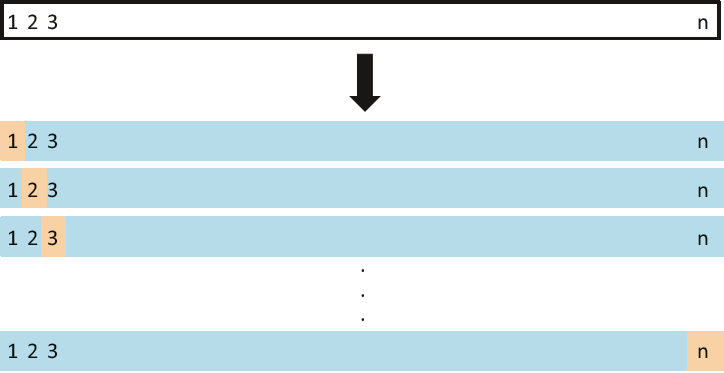
\includegraphics[width=0.5\linewidth]{crossValidation/LOOCV}
	\caption{}
	\label{fig:loocv}
\end{figure}


\begin{align}\label{fo:LOOCV}
CV_{(n)} = \frac {1}{n} \sum_{k=1}^{K}  (\frac {y_i-\hat{y_i}}{1- h_i})^2
\end{align}



\subsection{Result}
In lab 3.4.2 we had the same auto data. We used the LOOCV method to find MSE. We made an algorithm for this method, because we coul not find a library for this method.

\begin{lstlisting}[language=Python]
X = df["horsepower"].values.reshape(-1,1)
y = df["mpg"].values.reshape(-1,1) 

loo = LeaveOneOut()
print('Splits: ', loo.get_n_splits(X))

ytests = []
ypreds = []

for train_index, test_index in loo.split(X):
X_train, X_test = X[train_index], X[test_index]
y_train, y_test = y[train_index], y[test_index]

model = linear_model.LinearRegression()
model.fit(X = X_train, y = y_train)
y_pred = model.predict(X_test)

ytests += list(y_test)
ypreds += list(y_pred)

rr = metrics.r2_score(ytests, ypreds)
ms_error = metrics.mean_squared_error(ytests, ypreds)

print("LOOCV results:")
print("R^2: {:.5f}%, MSE: {:.5f}".format(rr*100, ms_error))
\end{lstlisting}

The output:
\begin{lstlisting}[language=Python]
Splits:  392
LOOCV results:
R^2: 60.12110%, MSE: 24.23151
\end{lstlisting}

As we can see our algorithm has worked.Also we have seen a mass increased computing time in the machine. It was expected, because of retraining and revalidating the model 392 time.